\documentclass[ignorenonframetext,]{beamer}
\usetheme{CambridgeUS}
\usecolortheme{sidebartab}
\setbeamertemplate{caption}[numbered]
\setbeamertemplate{caption label separator}{:}
\setbeamercolor{caption name}{fg=normal text.fg}
\usepackage{amssymb,amsmath}
\usepackage{ifxetex,ifluatex}
\usepackage{fixltx2e} % provides \textsubscript
\usepackage{lmodern}
\ifxetex
  \usepackage{fontspec,xltxtra,xunicode}
  \defaultfontfeatures{Mapping=tex-text,Scale=MatchLowercase}
  \newcommand{\euro}{€}
\else
  \ifluatex
    \usepackage{fontspec}
    \defaultfontfeatures{Mapping=tex-text,Scale=MatchLowercase}
    \newcommand{\euro}{€}
  \else
    \usepackage[T1]{fontenc}
    \usepackage[utf8]{inputenc}
      \fi
\fi
% use upquote if available, for straight quotes in verbatim environments
\IfFileExists{upquote.sty}{\usepackage{upquote}}{}
% use microtype if available
\IfFileExists{microtype.sty}{\usepackage{microtype}}{}
\usepackage{color}
\usepackage{fancyvrb}
\newcommand{\VerbBar}{|}
\newcommand{\VERB}{\Verb[commandchars=\\\{\}]}
\DefineVerbatimEnvironment{Highlighting}{Verbatim}{commandchars=\\\{\}}
% Add ',fontsize=\small' for more characters per line
\usepackage{framed}
\definecolor{shadecolor}{RGB}{248,248,248}
\newenvironment{Shaded}{\begin{snugshade}}{\end{snugshade}}
\newcommand{\KeywordTok}[1]{\textcolor[rgb]{0.13,0.29,0.53}{\textbf{{#1}}}}
\newcommand{\DataTypeTok}[1]{\textcolor[rgb]{0.13,0.29,0.53}{{#1}}}
\newcommand{\DecValTok}[1]{\textcolor[rgb]{0.00,0.00,0.81}{{#1}}}
\newcommand{\BaseNTok}[1]{\textcolor[rgb]{0.00,0.00,0.81}{{#1}}}
\newcommand{\FloatTok}[1]{\textcolor[rgb]{0.00,0.00,0.81}{{#1}}}
\newcommand{\CharTok}[1]{\textcolor[rgb]{0.31,0.60,0.02}{{#1}}}
\newcommand{\StringTok}[1]{\textcolor[rgb]{0.31,0.60,0.02}{{#1}}}
\newcommand{\CommentTok}[1]{\textcolor[rgb]{0.56,0.35,0.01}{\textit{{#1}}}}
\newcommand{\OtherTok}[1]{\textcolor[rgb]{0.56,0.35,0.01}{{#1}}}
\newcommand{\AlertTok}[1]{\textcolor[rgb]{0.94,0.16,0.16}{{#1}}}
\newcommand{\FunctionTok}[1]{\textcolor[rgb]{0.00,0.00,0.00}{{#1}}}
\newcommand{\RegionMarkerTok}[1]{{#1}}
\newcommand{\ErrorTok}[1]{\textbf{{#1}}}
\newcommand{\NormalTok}[1]{{#1}}
\usepackage{url}
\usepackage{graphicx}
\makeatletter
\def\maxwidth{\ifdim\Gin@nat@width>\linewidth\linewidth\else\Gin@nat@width\fi}
\def\maxheight{\ifdim\Gin@nat@height>\textheight0.8\textheight\else\Gin@nat@height\fi}
\makeatother
% Scale images if necessary, so that they will not overflow the page
% margins by default, and it is still possible to overwrite the defaults
% using explicit options in \includegraphics[width, height, ...]{}
\setkeys{Gin}{width=\maxwidth,height=\maxheight,keepaspectratio}

% Comment these out if you don't want a slide with just the
% part/section/subsection/subsubsection title:
\AtBeginPart{
  \let\insertpartnumber\relax
  \let\partname\relax
  \frame{\partpage}
}
\AtBeginSection{
  \let\insertsectionnumber\relax
  \let\sectionname\relax
  \frame{\sectionpage}
}
\AtBeginSubsection{
  \let\insertsubsectionnumber\relax
  \let\subsectionname\relax
  \frame{\subsectionpage}
}

\setlength{\parindent}{0pt}
\setlength{\parskip}{6pt plus 2pt minus 1pt}
\setlength{\emergencystretch}{3em}  % prevent overfull lines
\setcounter{secnumdepth}{0}
\usepackage{multicol}
\usepackage{graphicx}

\title{Survival Analysis using R}
\author{Phillip Ayieko}
\date{}

\begin{document}
\frame{\titlepage}

\begin{frame}{Survival Topics}

\begin{itemize}
\itemsep1pt\parskip0pt\parsep0pt
\item
  Survival Analysis concepts
\item
  Common survival analysis techniques
\item
  Presenting results
\item
  Both theory and practice

  \begin{itemize}
  \itemsep1pt\parskip0pt\parsep0pt
  \item
    Definitions
  \item
    censoring
  \item
    Kaplan-Meier
  \item
    Log-rank
  \item
    Cox proportional hazards
  \item
    R statistical software (open source:
    \url{http://cran.r-project.org/})
  \end{itemize}
\end{itemize}

\end{frame}

\begin{frame}{Introduction to survival analysis}

\begin{itemize}
\itemsep1pt\parskip0pt\parsep0pt
\item
  Survival Analysis is referred to statistical methods for analyzing
  survival/ time to event data
\item
  Events could be

  \begin{itemize}
  \itemsep1pt\parskip0pt\parsep0pt
  \item
    Recurrence of disease, death etc
  \end{itemize}
\item
  Examples

  \begin{itemize}
  \itemsep1pt\parskip0pt\parsep0pt
  \item
    Time between surgery and relapse
  \end{itemize}
\item
  Data is usually censored

  \begin{itemize}
  \itemsep1pt\parskip0pt\parsep0pt
  \item
    Example-study ends before all the patients dies
  \end{itemize}
\end{itemize}

\end{frame}

\begin{frame}{Objective of survival analysis}

\begin{itemize}
\itemsep1pt\parskip0pt\parsep0pt
\item
  Estimate probability that an individual surpasses some time-to-event
  for a group of individuals.
\item
  Compare time-to-event between two or more groups.
\item
  Assess the relationship of covariates to time-to-event.
\end{itemize}

\end{frame}

\begin{frame}{Types of survival data}

\begin{itemize}
\itemsep1pt\parskip0pt\parsep0pt
\item
  When the time of event is known, then we have complete information
  e.g.~rat number 4 died on 3rd day. This is called uncensored data
\item
  When the occurrences of the event are not known then we have
  incomplete information e.g.~those rats who escaped. This is called
  censored data
\item
  Follow-up time, calculated from

  \begin{itemize}
  \itemsep1pt\parskip0pt\parsep0pt
  \item
    exit time when the outcome is experienced, or last-seen time
  \item
    entry time when individual enters study
  \end{itemize}
\end{itemize}

\end{frame}

\begin{frame}{Two reasons for censoring}

\begin{itemize}
\itemsep1pt\parskip0pt\parsep0pt
\item
  During investigation we have incomplete information due to LOSS TO
  FOLLOW UP
\item
  When the investigation has come to an end and the experimental units
  are still alive. This is censoring due to WITHDRAWAL ALIVE
\end{itemize}

\end{frame}

\begin{frame}{Forms/ Types of censoring}

\begin{itemize}
\itemsep1pt\parskip0pt\parsep0pt
\item
  Right censoring
\item
  Left censoring
\item
  Type I censoring
\item
  Type II censoring
\item
  Random censoring
\item
  Interval censoring
\item
  Informative and non-informative censoring

  \begin{itemize}
  \itemsep1pt\parskip0pt\parsep0pt
  \item
    Most common is right censored
  \end{itemize}
\end{itemize}

\end{frame}

\begin{frame}{Censoring}

\begin{itemize}
\itemsep1pt\parskip0pt\parsep0pt
\item
  How could we account for censoring?

  \begin{itemize}
  \itemsep1pt\parskip0pt\parsep0pt
  \item
    Ignore it and say event occurred at time of censoring

    \begin{itemize}
    \itemsep1pt\parskip0pt\parsep0pt
    \item
      Incorrect because this is almost certainly not true
    \end{itemize}
  \item
    Remove patient from analysis

    \begin{itemize}
    \itemsep1pt\parskip0pt\parsep0pt
    \item
      Potential bias and loss of power
    \end{itemize}
  \item
    Survival analysis
  \end{itemize}
\item
  The objective is to estimate the survival distribution of patients in
  the presence of censoring
\end{itemize}

\end{frame}

\begin{frame}{Functions describing survival times}

\begin{itemize}
\item
  T is a random variable representing survival time - Can be described
  by a probability distribution

  \begin{itemize}
  \itemsep1pt\parskip0pt\parsep0pt
  \item
    1.Cumulative distribution function
  \item
    2.Survival function
  \item
    3.Probability density function
  \item
    4.Hazard function
  \item
    5.Cumulative hazard function
  \end{itemize}
\end{itemize}

\end{frame}

\begin{frame}{Functions of T}

\begin{itemize}
\itemsep1pt\parskip0pt\parsep0pt
\item
  Let \textbf{T} denote the survival time
\item
  \(t \equiv\) a specific point in time.
\end{itemize}

\begin{enumerate}
\def\labelenumi{\arabic{enumi}.}
\itemsep1pt\parskip0pt\parsep0pt
\item
  \textbf{Survival function}
\end{enumerate}

\begin{itemize}
\item
  \(s(t)=p(surving\_longer_than\_time\_t)\)
\item
  Survival function: probability survival time is greater than a
  specific value \(S(t)=P(T>t)\)
\item
  \(S=\frac{number\_of_patients\_surviving\_longer\_than\_t}{total\_number\_of\_patients\_in\_the\_study}\)
\end{itemize}

\end{frame}

\begin{frame}{Mathematical Definitions}

\begin{itemize}
\item
  Distribution function \[
   F(t)=Pr(T\leq t)
  \]
\item
  Density Function \[
  f(t)=\frac{\partial{F(t)}}{\partial{t}}
  \]
\item
  Survival Function \[
  S(t)=Pr(T>t)=1-F(t)
  \]
\end{itemize}

\end{frame}

\begin{frame}{Mathematical Definitions}

\begin{itemize}
\itemsep1pt\parskip0pt\parsep0pt
\item
  Hazard function: \[
  h(t)=\lim_{\Delta t \to 0} \frac{Pr(t\leq T \leq t + \Delta t|T\geq t)}{\Delta t} = \frac{f(t)}{S(t)}
  \]
\item
  Cumulative hazard
\end{itemize}

\[
H(t)=\int_{0}^{t} h(u) du
\]

\end{frame}

\begin{frame}{Statistical Inference}

\begin{itemize}
\itemsep1pt\parskip0pt\parsep0pt
\item
  Has two components

  \begin{itemize}
  \itemsep1pt\parskip0pt\parsep0pt
  \item
    Estimation of survival function
  \item
    Testing of hypothesis of survival functions
  \end{itemize}
\item
  There are two methods of approaching them

  \begin{itemize}
  \itemsep1pt\parskip0pt\parsep0pt
  \item
    Parametric approach
  \item
    Non parametric approach
  \end{itemize}
\item
  A combination of the 2 approaches gives the regression
  (i.e.~estimation and testing of the hypothesis)
\end{itemize}

\end{frame}

\begin{frame}{KAPLAN-MEIER ESTIMATOR}

\end{frame}

\begin{frame}{Kaplan-Meier Estimate of S(t)}

\begin{itemize}
\item
  Kaplan-Meier estimator of survival is a nonparametric method of
  inference concerning the survivor function \(S = Pr(T > t)\)
\item
  Rank the survival times as \(t_1 \leq t_2 \leq ... \leq t_n\)
\item
  Number of individuals at risk before \(t_i \equiv n_i\)
\item
  Number of individuals with failure time \(t_i \equiv d_i\)
\item
  Estimated hazard function at \(t_i\): \(h_i=\frac{d_i}{n_i}\)
\item
  Formula \[
  S(t) = \prod_{t_i \leq t} \frac{n_i - d_i}{n_i}
  \]
\end{itemize}

\end{frame}

\begin{frame}{Kaplan-Meier Estimate of S(t)}

\[
var[s(t)]\approx [s(t)]^2\sum \frac{d_j}{n_j(n_j-d_j)}
\]

\begin{itemize}
\itemsep1pt\parskip0pt\parsep0pt
\item
  And the 95 \% CI is given by
\end{itemize}

\[
s(t)\pm 1.96 \sqrt{var(s(t))}
\]

\end{frame}

\begin{frame}{Kaplan-Meier Curve}

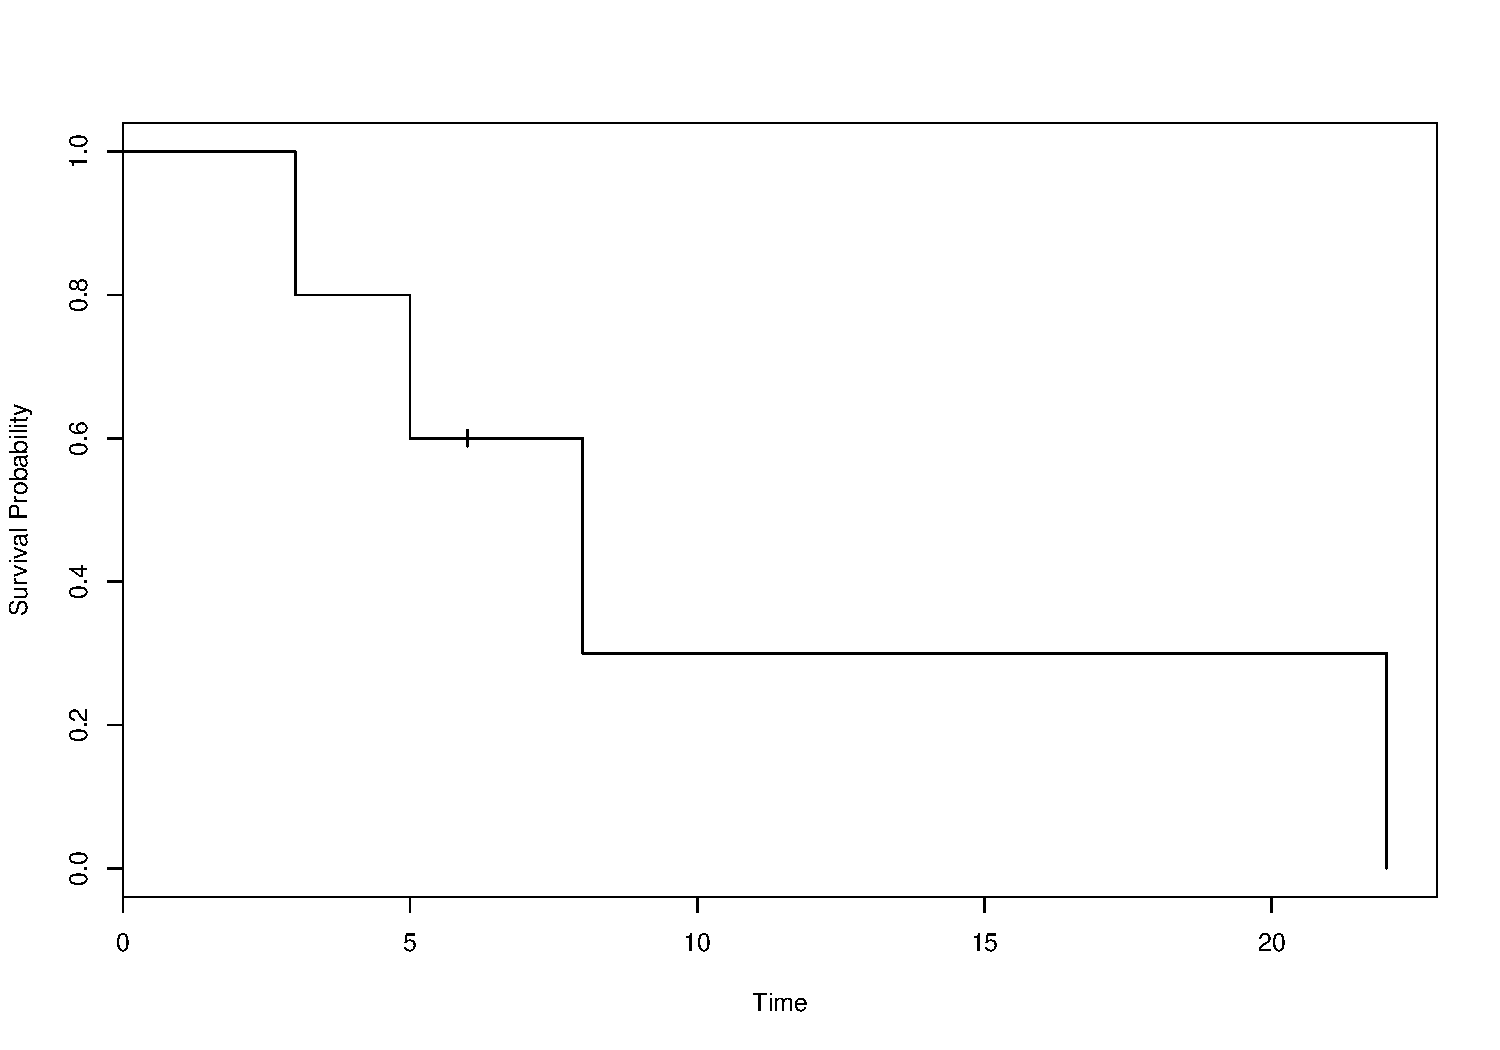
\includegraphics{survival_analysis_files/figure-beamer/unnamed-chunk-1-1.pdf}

\end{frame}

\begin{frame}{Functions of interest in R}

\begin{itemize}
\itemsep1pt\parskip0pt\parsep0pt
\item
  Survival object: \textbf{Surv}
\item
  Kaplan-Meier estimates: \textbf{survfit}
\item
  The log-rank test: \textbf{survdiff}
\item
  The Cox proportional hazards model: \textbf{coxph}
\item
  The Accelerated failure time model: \textbf{survreg}
\item
  Relevant R packages: \textbf{survival, survcomp, HMISC, Design, MASS}
\end{itemize}

\end{frame}

\begin{frame}{Example}

\begin{itemize}
\itemsep1pt\parskip0pt\parsep0pt
\item
  Event = time to relapse
\item
  Data:

  \begin{itemize}
  \itemsep1pt\parskip0pt\parsep0pt
  \item
    10, 20+, 35, 40+, 50+, 55, 70+, 71+, 80, 90+
  \end{itemize}
\item
  Before complex functions may be performed, the data has to be put into
  the proper format: a \textbf{survival object}
\item
  In R we use \textbf{Surv(time, status)}
\item
  \emph{time} is a vector of event time, and \emph{status} is a vector
  of indicator (denoting if the event was observed or censored
\end{itemize}

\end{frame}

\begin{frame}[fragile]{R codes for Kaplan-Meier}

\begin{Shaded}
\begin{Highlighting}[]
\KeywordTok{library}\NormalTok{(survival)}

\NormalTok{time <-}\StringTok{ }\KeywordTok{c}\NormalTok{(}\DecValTok{10}\NormalTok{,}\DecValTok{20}\NormalTok{,}\DecValTok{35}\NormalTok{,}\DecValTok{40}\NormalTok{,}\DecValTok{50}\NormalTok{,}\DecValTok{55}\NormalTok{,}\DecValTok{70}\NormalTok{,}\DecValTok{71}\NormalTok{,}\DecValTok{80}\NormalTok{,}\DecValTok{90}\NormalTok{)}
\NormalTok{status <-}\StringTok{ }\KeywordTok{c}\NormalTok{(}\DecValTok{1}\NormalTok{,}\DecValTok{0}\NormalTok{,}\DecValTok{1}\NormalTok{,}\DecValTok{0}\NormalTok{,}\DecValTok{0}\NormalTok{,}\DecValTok{1}\NormalTok{,}\DecValTok{0}\NormalTok{,}\DecValTok{0}\NormalTok{,}\DecValTok{1}\NormalTok{,}\DecValTok{0}\NormalTok{)}
\NormalTok{data <-}\StringTok{ }\KeywordTok{data.frame}\NormalTok{(time,status)}

\NormalTok{survobj <-}\StringTok{ }\KeywordTok{with}\NormalTok{(data,}\KeywordTok{Surv}\NormalTok{(time,status))}

\NormalTok{fit <-}\StringTok{ }\KeywordTok{survfit}\NormalTok{(survobj~}\DecValTok{1}\NormalTok{, }\DataTypeTok{data=}\NormalTok{data)}
\NormalTok{fit}
\end{Highlighting}
\end{Shaded}

\begin{verbatim}
## Call: survfit(formula = survobj ~ 1, data = data)
## 
## records   n.max n.start  events  median 0.95LCL 0.95UCL 
##      10      10      10       4      80      55      NA
\end{verbatim}

\begin{Shaded}
\begin{Highlighting}[]
\KeywordTok{summary}\NormalTok{(fit)}
\end{Highlighting}
\end{Shaded}

\begin{verbatim}
## Call: survfit(formula = survobj ~ 1, data = data)
## 
##  time n.risk n.event survival std.err lower 95% CI upper 95% CI
##    10     10       1    0.900  0.0949       0.7320            1
##    35      8       1    0.787  0.1340       0.5641            1
##    55      5       1    0.630  0.1770       0.3632            1
##    80      2       1    0.315  0.2397       0.0709            1
\end{verbatim}

\begin{Shaded}
\begin{Highlighting}[]
\KeywordTok{attributes}\NormalTok{(fit)}
\end{Highlighting}
\end{Shaded}

\begin{verbatim}
## $names
##  [1] "n"         "time"      "n.risk"    "n.event"   "n.censor" 
##  [6] "surv"      "type"      "std.err"   "upper"     "lower"    
## [11] "conf.type" "conf.int"  "call"     
## 
## $class
## [1] "survfit"
\end{verbatim}

\end{frame}

\begin{frame}[fragile]

\begin{Shaded}
\begin{Highlighting}[]
\KeywordTok{plot}\NormalTok{(fit, }\DataTypeTok{xlab=}\StringTok{"time to relapse (months)"}\NormalTok{, }\DataTypeTok{ylab=}\StringTok{"Survival Function"}\NormalTok{, }\DataTypeTok{yscale=}\DecValTok{100}\NormalTok{, }\DataTypeTok{main=}\StringTok{"Survival Distribution"}\NormalTok{)}
\end{Highlighting}
\end{Shaded}

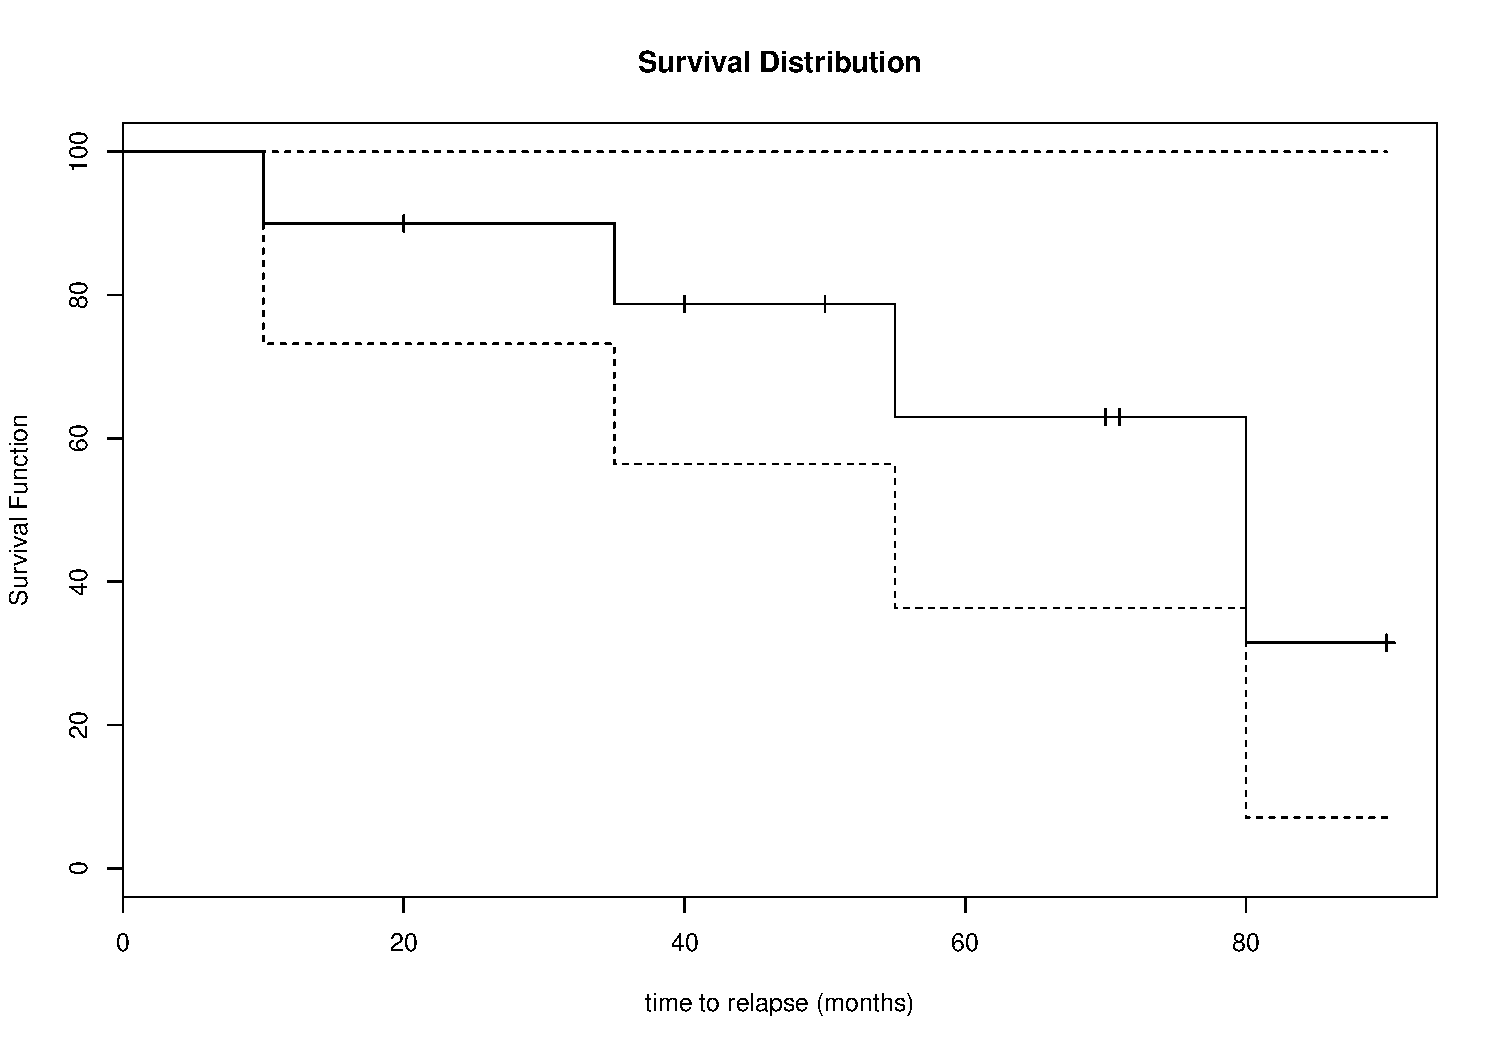
\includegraphics{survival_analysis_files/figure-beamer/unnamed-chunk-3-1.pdf}

\end{frame}

\begin{frame}[fragile]{Aalen-Nelson Estimate of S(t)}

\begin{itemize}
\itemsep1pt\parskip0pt\parsep0pt
\item
  Uses the cumulative hazard function \[
  H(t) = - \log s(t) = \sum_{t_j\leq t}\frac{d_j}{n_j}
  \]
\end{itemize}

\[
s(t)=e^{-\int_{0}^{t} h(u)d(u)} =e^{-H(t)}
\]

\begin{itemize}
\itemsep1pt\parskip0pt\parsep0pt
\item
  In R, to estimate S(t), using output from \emph{survfit()}
\end{itemize}

\begin{Shaded}
\begin{Highlighting}[]
\CommentTok{#survobj <- Surv(time, status)}
\CommentTok{#fit1 <- summary(survfit(survobj~1))}
\CommentTok{# S.hat <- fit1$surv}
\CommentTok{# H.hat <- -log(S.hat)}
\CommentTok{#a<- survfit(coxph(Surv(time,status)~1), type="aalen")}
\CommentTok{#summary(a)}
\CommentTok{#basehaz(coxph(Surv(time,status)~1,data=data))}
\end{Highlighting}
\end{Shaded}

\end{frame}

\begin{frame}{LOG-RANK TEST}

\end{frame}

\begin{frame}{LOG-RANK TEST}

\begin{itemize}
\item
  Use the Log-Rank Test to compare the survival functions of two
  samples/ treatment groups.
\item
  \(H_0\): The two survival functions are the equivalent
\item
  \(H_a\): The two survival functions are different
\item
  Goal: Test whether two groups differ in population survival functions.
\end{itemize}

\end{frame}

\begin{frame}{Log-Rank Test}

\begin{itemize}
\itemsep1pt\parskip0pt\parsep0pt
\item
  Notation:
\item
  \(t_{i} \equiv\) Time of the ith failure time (across groups)
\item
  \(d_{1i} \equiv\) number of failures for trt 1 at time \(t_{(i)}\)
\item
  \(d_{2i} \equiv\) Number of failures for trt 2 at time \(t_{(i)}\)
\item
  \(n_{1i} \equiv\) Number at risk prior for trt 1 prior to time
  \(t_{(i)}\)
\item
  \(n_{2i}\) Number at risk prior for trt 2 prior to time \(t_{(i)}\)
\end{itemize}

\(d_i = d_{1i}+ d_{2i}\) and \(n_i=n_{1i}+n_{2i}\) \[
v_{li} =\frac{ n_{1i}n_{2i}d_i(n_i-d_i) }{n_{i}^{2} (n_i-1)}
\]

\[
e_{1i} = \frac {n_{1i} d_{1i}}{n_i}
\]

\[
O_1-E_1 =\sum_i (d_{1i}-e_{1i})
\]

\[
V_1=\sum_i v_{li}
\]

\end{frame}

\begin{frame}[fragile]{R codes}

\begin{Shaded}
\begin{Highlighting}[]
\KeywordTok{survdiff}\NormalTok{(formula, }\DataTypeTok{rho=}\DecValTok{0}\NormalTok{)}
\end{Highlighting}
\end{Shaded}

\begin{itemize}
\itemsep1pt\parskip0pt\parsep0pt
\item
  \emph{formula} is a survival object against a categorical covariate
  variable.
\item
  \emph{rho} is a scalar parameter that controls the type of test.
\item
  With default \emph{rho=0}, this is the log-rank or Mantel-Haenszel
  test.
\item
  With \emph{rho=1}, it is equivalent to the Peto and Peto modi???cation
  of the Gehan-Wilcoxon test.
\end{itemize}

\begin{Shaded}
\begin{Highlighting}[]
  \NormalTok{>}\KeywordTok{survdiff}\NormalTok{(survobj~status, }\DataTypeTok{rho=}\DecValTok{0}\NormalTok{)}
\end{Highlighting}
\end{Shaded}

\end{frame}

\begin{frame}{Cox Proportional Hazard Model}

\end{frame}

\begin{frame}{Cox Proportional Hazard Model}

\begin{itemize}
\itemsep1pt\parskip0pt\parsep0pt
\item
  CPHM is a technique for investigating the relationship between
  survival time and independent variables
\item
  The most popular model for survival analysis:
\item
  Goal: Compare two or more groups (treatments), adjusting for other
  risk factors on survival times (like Multiple regression)
\item
  p explanatory variables (including dummy variables)
\end{itemize}

\end{frame}

\begin{frame}{Cox regression for time to event}

\begin{itemize}
\item
  Useful when incidence rates vary over time
\item
  hazards in both exposed and unexposed are allowed to vary but their
  ratio is assumed to be constant - this is the proportional hazards
  assumption. Thus the Cox model are also known as the proportional
  hazards model
\item
  Cox model is fitted by creating risk sets of individuals still at risk
  at the time of each failure
\end{itemize}

\end{frame}

\begin{frame}{Cox Proportional Hazard Model}

\begin{itemize}
\item
  The semi-parametric model given by \[
  h_i(t)=h_0(t)\exp(\beta_1 x_{i1} + \beta_2 x_{i2} + ... + \beta_k x_{ik})
  \]
\item
  \(h_0(t)\) is the baseline hazard function. This is the function when
  all the covariates equal to zero
\item
  The hazard ratio is independent of time t. \[
  HR_{i,j}=\frac{h_i(t)}{h_i(t)} +\frac{\lambda_0(t)e^{\beta_1 x_{i1} + ... + \beta_k x_{ik}}} { \lambda_0(t)e^{\beta_k x_{j1} + ... + \beta_k x_{jk}}} = e^{\beta_1 x_{j1} + ... + \beta_k x_{jk}}
  \]
\end{itemize}

-This defines the \textbf{proportional hazards property}

\end{frame}

\begin{frame}{Interpretation of the Betas}

\begin{itemize}
\itemsep1pt\parskip0pt\parsep0pt
\item
  We need to find the ratio where there is a unit increase in the
  covariates provided other covariates stay fixed
\end{itemize}

\[
\frac{h(t,x_1+1)}{h(t,x_1)} = \frac{h_0(t)e^{\beta_1(x_1+1)}}{h_0(t)e^{\beta_1(x_1)}} = e^{\beta_1}
\]

\begin{itemize}
\itemsep1pt\parskip0pt\parsep0pt
\item
  We interprete as the unit increase in log hazard per unit increase of
  x
\item
  (just as log-odds in logistic regression)
\end{itemize}

\end{frame}

\begin{frame}{R example}

\begin{itemize}
\itemsep1pt\parskip0pt\parsep0pt
\item
  \(> coxph(formula, method)\)
\item
  \textbf{formula} is linear model with a survival object as the
  response variable
\item
  \textbf{method} is used to specify how to handle ties. The default is
  `efron'. Other options are `breslow' and `exact'.
\item
  \(> cox.fit < -coxph(Surv(time, status) x+y+z, method =‘breslow)\)
\item
  to obtain the baseline survival function
  \(> my.survfit.object <- survfit(coxph.fit)\)
\end{itemize}

\end{frame}

\end{document}
